\documentclass[12pt,letterpaper]{article}
\usepackage{graphicx}

\usepackage[margin=1in]{geometry}

\begin{document}

\begin{flushright}
Homework 3: Profile Guided Optimization\\
Paul Vines and Eric Mullen\\
CSE 501\\
\end{flushright}

\subsection*{How To Run:}
\emph{Compile: (Scala Compiler Version 2.10.1)}\\
In code directory: scalac *.scala\\

\emph{Run:}\\
In test or untyped directory: run.sh [-opt=OPTIONS] filename\\
OPTIONS: ssa, cse, scp, cbr, dtr, mem\\
cse, cbr, and scp will not run without also specifying ssa\\


\subsection*{Optimizations}
\subsubsection*{Dynamic Type Refinement}
The purpose of the Dynamic Type Refinement (DTR) optimization is to
attempt to eliminate dynamic loads and stores via profile-based
optimization. Dynamic loads and stores can make up a significant
amount (up to 50\% in the example programs) of the run-time of a
program, so reducing them is a potentially high-value target for
optimization.
The profiling is conducted by inserting a counter before
each dynamic load and store instruction to track which type the
object is that is used in the dynamic instruction. These counts are
gathered and any count showing that only a single type is ever used at
a certain position is marked for optimization. Since the type of the
object being operated on is known, the exact offset (and type of the
value loaded, if it is a dynamic load) can be determined. 
To optimize a dynamic load, the lddynamic instruction is converted
into a load preceded by an add to create the proper address from the
object address and offset. Additionally, if the type of the expected
return value is a primitive then the subsequent unboxing instructions
are deleted since the load instruction will automatically unbox the
primitive.
To optimize a dynamic store is simpler; this only requires replacing
the stdynamic instruction with an add and store to the proper address
offset.
The results of this optimization are impressive for the programs it
works on: class, untyped\_class, and untyped\_struct all show
significant improvements, with untyped\_class and untyped\_struct
runtimes being more than cut in half. 
\begin{center}
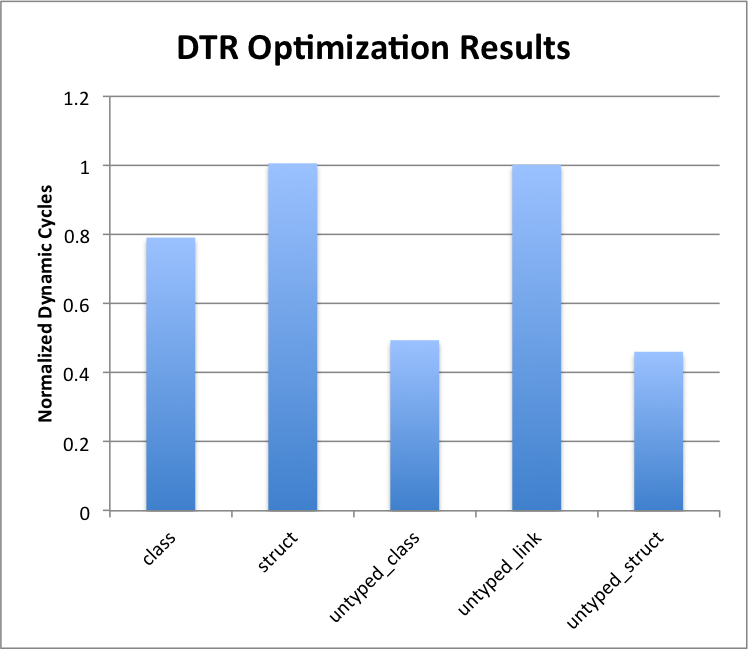
\includegraphics[width=4in]{dtrstats.png}
\end{center}

\subsubsection*{Code Layout}

This optimization is enabled with the option ``cbr''. It will not work
if ``ssa'' is not also specified.

Here, we aim to improve the layout of basic blocks in memory by
counting how many times branches are taken in the code. First, we
instrument all unconditional branches with a counter, and instrument
each conditional branch with two counters. We do this while the code
is in SSA form, which is also the point in our code where all
transitions between basic blocks are explicit, i.e. there are no
points where we simply fall off the end of a basic block into the next
basic block. These counters are then used as the priorities of the
basic blocks when they are layed out in each function. Previously,
blocks were layed out in an arbitrary topological sort, now they are
layed out in a priority topological sort. The only difference is,
instead of a worklist, a priority queue is used to keep the blocks
currently being processed, and thus higher priority blocks (those on
the hot code path) are all layed out close to each other.

This has surprisingly little effect on runtime, in most cases leaving
the optimized program with the exact same dynamic cycle count as its
non-optimized version. In the cases where the runtime is not the same,
the optimized code ends up running slightly slower. We are not
entirely sure what causes this. These results confirmed our hypothesis
that code layout was not an especially large factor in program
runtime, and that the original order a program is written in is in
fact not that bad as a basic block layout.


\subsubsection*{Output Memoization}

This optimization is enabled by the ``mem'' option.

This optimization runs the program, and grabs all output the program
produces. It then constructs a program that is a series of
instructions that writes the same output, and produces that as its
optimized program.

This optimization is provably optimal, if we consider program
equivalence as only an I/O equivalence, i.e. two programs are
equivalent if and only if they produce the same output. We noticed the
key point that Start has no capacity for input (other than constants
hard coded into the program text), and has only the capacity to write
integers and newline characters to the screen. Thus, if we have some
input program that produces some output when run, there is an infinite
set of programs that produce the same output when run. However, one of
these programs is optimal, in that it does no other computational work
other than that required to produce the output. As there is only one
way for a Start program to produce a specific output, the program that
produces this output and computes nothing is thus optimal, in that it
will run in a shorter amount of time than any other equivalent program
in this set.

This does not work if the program does not halt. However, for us to
apply a profile guided optimization, we are already making the
assumption that the program halts, and none of our profile guided
optimizations work if this assumption breaks.

In practice this optimization garners a massive speedup on any program
that isn't a series of print statements. This is still of limited use
in any useful setting, as most languages that exist in the wild have
the capacity for input to their programs.

\begin{center}
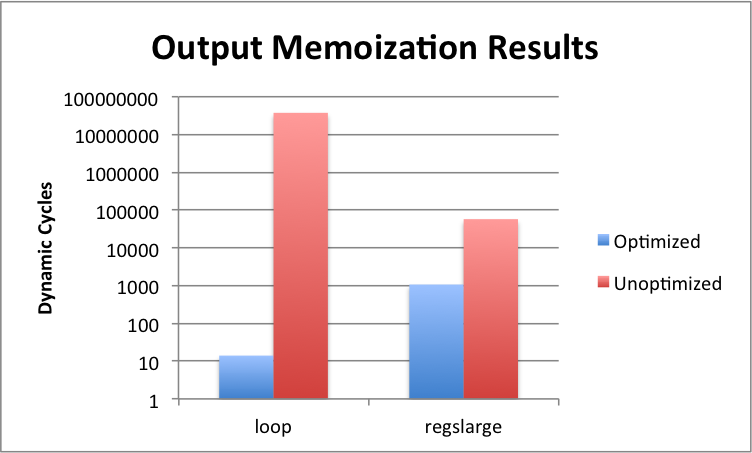
\includegraphics[width=4in]{memostats.png}
\end{center}

\subsection*{Code Statistics}

Our final implementation is 2443 lines of Scala in 12 files. When
compiled, they generate 612 distinct Java class files. 

\end{document}
